% chktex-file 44
% chktex-file 29
% chktex-file 8
\documentclass{rhumj_new}
\usepackage{amsmath} \usepackage{float}
\usepackage{collcell} \newcommand{\fwcell}[1]{\makebox[\arraystretch\normalbaselineskip]{$#1$}}

\graphicspath{{./images/}}

\title[Magic Squares]{An Approach to Computing Magic Squares Using High-Performance Computing and
  Group Theory}

\author[Keough]{Nathan H. Keough
  \thanks{Thank you to my friends, peers, and professors for allowing and
    encouraging me to succeed.}}
\affiliation{Maryville College}
\email{nathan.keough@my.maryvillecollege.edu}

%additional authors; list in alphabetical order by last name
% \author[Euler]{Leonard Euler\thanks{Thanks for nothing, Bernoulli.}}
% \affiliation{University of Basel}
% \email{oiler@notmail.com}

%please include 2010 mathematics subject classification:
%https://mathscinet.ams.org/msc/msc2010.html
% Computer science {For papers containing software, source code, etc. in a specific mathematical area, see the classification number –04 in that area}
\subjclass{68V99}
%please provide keywords for your article
\keywords{magic squares, computational group theory, rust}

%\abstract{A brief abstract goes here.}

\begin{document}
\newpage{}
\abstract{\
  This paper introduces a novel algorithm for computing magic squares, exploiting group theory
  concepts such as permutation representation, group operations, and group actions to encode
  symmetries. By defining the group operation as composition, we may systematically explore the
  permutations of the group and extrapolate information about the magic squares to generate new
  magic
  squares not in the originating set. This vastly reduces computation times for enumerating the
  solutions to magic squares, while also encoding the symmetries in a manner that is easier to
  analyze programmatically. Overall, this study reveals the profound connection between magic
  squares
  and group theory, offering promising avenues for symmetry-driven algorithms and applications in
  combinatorial mathematics.
}
\newpage{}
\section{Introduction}

\begin{figure}[ht!]
  \begin{align*}
    \quad \renewcommand{\arraystretch}{2}
    \begin{tabular}{|
      *{3}{>{\collectcell\fwcell}c<{\endcollectcell} |} }
      \hline 2 & 9 & 4 \\
      \hline 7 & 5 & 3 \\
      \hline 6 & 1 & 8 \\
      \hline
    \end{tabular}
  \end{align*}
  \caption{The magic square of order 3 is shown.}\label{fig:square}
\end{figure}

The secrets behind magic squares have engaged mathematicians for millennia. The magic square
problem itself is believed to have originated in China around 2200 BCE with the introduction of
what are now known as “Lo-Shu” magic squares\cite{Cammann}. These magic squares are defined as
$3\times3$ grids with the numbers $1$ through $9$ arranged such that the sums of all the rows,
columns, and diagonals are the same. Note in Fig.~\ref{fig:square} that the rows, columns, and
diagonals each add to $15$.

This property is what makes a square ``magic,'' lending a connotation of power that is
respected by many ancient cultures. In many ways, magic squares have held a mythical reputation in
culture due to their unique properties. As mathematics evolved, so did the study of magic squares
worldwide, later appearing in India, The Middle East, and Latin Europe. Each rendition of the magic
square problem brings with it new questions in mathematics. The number of solutions to the Lo-Shu
magic square problem is well known. However, The number of solutions to other kinds of squares
remains a great mystery, especially as the size of the square grows.

Today, magic squares hold less of a mythical and powerful cultural reputation. Mathematics, at this
point in history, has been able to deduce new and creative uses for magic squares in various
different fields, especially physics. In 2021, scientists found a connection between electrostatic
potentials and magic squares of the $4^{th}$ and $5^{th}$ order\cite{Fahimi}. Similarly, magic
squares of the $6^{th}$ order have been associated with the Weak Force in physics\cite{ONeill}.
Outside of physics, there are also uses for magic squares in image encryption, specifically, using
large squares as chaos maps in chaos-based encryption schemes\cite{Wang}. For these reasons and
many others, the continual study of magic squares carries with it the possibility of new
breakthroughs in applied mathematics.

Although there are many kinds of magic squares, we will only interest ourselves in ``normal''
magic squares, which have two main requirements: $(1)$ The square must be filled with the integers
from $1$ to $n^2$ inclusive, where $n$ is the order of the magic square, and $(2)$ the sums of the
main columns, rows, and diagonals must equal the same integer. This integer $S$ is called the
``magic sum'' and is calculated by $nS = \frac{n^2(n^{2}+1)}{2}$ with the right-hand side equating
to the sum of the first $n^2$ positive integers, and the left-hand side equal to the magic sum
multiplied by a factor $n$, the order of the square. Dividing by this factor on both sides
satisfies this equation for the magic sum. The number of rows, columns, and diagonals is equal to
$2n+2$ with $n$ being the order of the square. This is considered the number of ``constraint
vectors'' of a magic square.

\begin{figure}[ht!]
  \begin{align*}
    \quad \renewcommand{\arraystretch}{2}
    \begin{tabular}{|
      *{3}{>{\collectcell\fwcell}c<{\endcollectcell} |} }
      \hline 2 & 9 & 4 \\
      \hline 7 & 5 & 3 \\
      \hline 6 & 1 & 8 \\
      \hline
    \end{tabular}
    \quad \renewcommand{\arraystretch}{2}
    \equiv
    \quad \renewcommand{\arraystretch}{2}
    \begin{tabular}{|
      *{3}{>{\collectcell\fwcell}c<{\endcollectcell} |} }
      \hline 6 & 7 & 2 \\
      \hline 1 & 5 & 9 \\
      \hline 8 & 3 & 4 \\
      \hline
    \end{tabular}
  \end{align*}
  \caption{The magic squares are isometric.}\label{fig:unique}
\end{figure}

We are also only interested in studying ``unique'' magic squares. By this, we mean magic
squares that are unique up to rotations and reflections or isometry. An example of this is taking a
magic square $A$ and rotating it $90^{\circ }$ or reflecting it about the y-axis any number of
times. The resulting square will always be considered equivalent to $A$. There may also be times
when we refer to a ``positionally distinct'' magic square. In this case, isometries of a magic
square $A$, result in a ``different'' square $B$. Neither of these definitions affect the validity
of magic squares; they only affect how we count them. Fig.~\ref{fig:unique} accurately represents
two magic squares that we would consider to be the ``same'' square up to isometry.

There is only one unique solution for the Lo-Shu Square, pictured in Fig.~\ref{fig:square}. There
are extensions to the magic square problem, with variants having larger side lengths (order),
different ``magic'' requirements, or different kinds of element values. For order four, there are
$880$ unique solutions. For order five, there are $275,305,224$ unique solutions\cite{Fahimi}.
However, the number of exact unique solutions for order six remains unknown. The number of unique
solutions for each order exhibits a kind of exponential growth, and their values have been of
interest to mathematicians and hobbyists since the puzzle's inception.

\subsection{Permutations}

The main mechanism that we use for encoding a magic square and its properties comes from Group
and Number Theory. Specifically, we will study the permutations of magic squares. In the 1770s,
Joseph Louis Lagrange studied permutations of the roots of polynomial equations. This led to Galois
theory founded by Évariste Galois, which describes what is or is not possible with respect to
solving polynomial equations by radicals\cite{Fraser}. In modern mathematics, there are many
similar
situations where studying permutations can help us understand a problem.

Roughly speaking, magic squares may be represented as permutations of $n^2$ objects. By the
definition of a normal magic square, these are the positive integers (mod $n^2$). The dimension
need not matter since the coordinates of elements in a two-dimensional, row-major grid square may
be mapped to a one-dimensional sequence, which is a bijection. The square, laid out as a
one-dimensional sequence, represents the sequence of integers as a permutation. There are a total
of $n^{2}$! permutations of a square, where $n$ is the order of the square. The permutations of
squares represent the different possible configurations of integers in the square, many of them
meeting the requirements to be considered magic squares.

\begin{figure}[ht!]
  \begin{align*}
    \quad \renewcommand{\arraystretch}{2}
    \begin{tabular}{|
      *{3}{>{\collectcell\fwcell}c<{\endcollectcell} |} }
      \hline a & b & c \\
      \hline d & e & f \\
      \hline g & h & i \\
      \hline
    \end{tabular}
  \end{align*}
  \caption{The set $S$ may be imagined as an $n\times n$ grid square.}\label{fig:squareperm}
\end{figure}

The concept of interpreting grid squares as permutations may be realized by
Fig.~\ref{fig:squareperm} where the set $S = \{a, b, c, d, e, f, g, h, i\} \in S_9$. By decomposing
the rows of an $n\times n$ square into an ordered set containing all elements from $1\cdots n^2$,
we may consistently map the set to unique permutations on $n^2$ objects.

We believe that by studying different permutations of squares, including those that are magic,
we may be able to describe various kinds of symmetry related to magic squares of specific orders.
Treating individual squares as permutations and vice-versa allows us to make use of the properties
relating to permutations in general, meaning we can perform unique transformations or actions on
them using methods originating from group theory. Additionally, we may define other mathematical
properties that allow us to better describe magic squares and their associated symmetries that go
beyond simple row and column transposition.

\subsection{Enumeration}

In our investigation into the inner structures and symmetries of magic squares, we may find it
useful to enumerate the magic squares, i.e.\ exhaustively listing and analyzing every magic square
of a specific order. By hand, this is difficult, but with high performance programming, we can do
this very easily for certain orders and with certain algorithms. Prior to modern computing,
mathematicians were computing large orders by hand using various methods. Some in particular
developed by W.S. Andrews in 1908 utilized ``constructions'', whereby assumptions about initial
known values are used to help complete a magic square using some algorithmic process, potentially
cutting down on the total amount of computation\cite{Andrews}. Some aspects of constructions are
similar to the method outlined in this paper but with some differences. Our method makes no
assumptions about initial values, but some code exists that could support constructive methods of
magic square generation. Listing magic squares in this way, as we will see, is useful and allows us
to generalize certain properties of magic squares, potentially also for higher orders.

Recall that the number of permutations of $n$ objects is $n$!. We can actually exploit this
fact to implement an element of ordering for magic squares. There exists a natural ordering from
$S_n$, the group of all permutations on $n$ elements, to $\mathbb{Z}^{*}_{n!-1}$  in the
factor-adic number system, (*) meaning non-negative. This number system, also known as the
factorial number system, is a mixed radix adapted for combinatorial systems. In this system, we can
express the permutations of $n$ objects in lexicographical order, that is naturally from $0$ to
$n!-1$ as a bijection. Using the factor-adic number system's properties we can treat magic squares
(or any grid square) as a permutation, and map that permutation uniquely to an integer. More
generally, this concept is called a Lehmer Encoding of a permutation on $n$ integers\cite{Lehmer}.
This
not only simplifies our intuition of what a unique magic square looks like, but also improves the
performance of a magic square computation in some cases, specifically, the cost of copying integers
over whole arrays and storing magic squares in memory.

It should be noted that the indices of magic squares in their ordered set do not follow an easily
identifiable pattern. Perhaps there is a pattern, but we have no way of identifying it based on our
current assumptions of magic squares. In any case, analyzing the frequency of magic squares in
their ordered set has not so far proved to be helpful. Exhaustive enumeration of magic squares is
presumed to be an NP-Hard problem, making it suitable for certain cryptographic applications.
However, it is at least NP;\@ the NP-completeness and classification of the magic square problem is
formally unknown. For context, P versus NP is an unsolved problem in theoretical computer science
and is a millennium prize problem. A problem classified as P is solvable and verifiable in
polynomial time with respect to its input size. Problems in NP are verifiable in polynomial time.
Solving if P = NP would mean that problems verifiable in polynomial time are solvable in polynomial
time. A problem X in NP is considered NP-complete if and only if any other problem in NP is
reducible to X. The class of NP-Hard problems contains all NP-Complete problems but also includes
those that are undecidable. The theoretical complexity of predicting magic squares is unknown, yet,
there do exist applications in artificial intelligence for predicting and classifying magic
squares\cite{Weed}. The role of artificial intelligence in mathematics is becoming increasingly
apparent. Opting for AI-driven solutions could be a great approach for future studies.

\section{Computational Approach}

\subsection{Introduction}

To help us compute magic squares, we have implemented a custom Computational Algebra System
(CAS) written in the Rust Programming Language. This system allows us to construct and manipulate
square data to find magic squares. Once we have magic squares, we may do additional processing on
them to learn more about their structures. The system is geared for high performance and thus
implements some of the best known strategies for working with magic square structures, both
mathematically and programmatically. The code itself is structured as a crate or library, so given sufficient
interest, it can be readily published. Alternatively, all the code is on GitHub\cite{Keough}.

In addition to the high-performance aspects of our code, we've also added features that would
be useful to other scientists exploring magic squares. Additional features include the ability to
log or serialize computations to files, encode magic squares in compressed formats, implement
parameter sets defining large-order squares, use constructive methods, and run examples with
extensive documentation.

All implementations are justified through the use of a benchmark-driven software development
policy, meaning certain implementations or algorithms are added, used, and possibly
modified based on benchmarking and profiling results. This, of course, is highly dependent on the
hardware being used. Our specific hardware being used to quantify and express the results of
computed magic squares includes:

\begin{itemize}
  \item AMD Ryzen 7 5800X x8 (16) @ 4.200GHz, 32 GB RAM \textemdash{}  Pop!\_Os 22.04 LTS x86\_64
  \item Apple M2 x8 (8) (x4 performance, x4 efficiency) @ 3.500GHz, 24 GB RAM \textemdash{} macOS
        13.3.1
        22E261 ARM64
\end{itemize}

\subsection{Modern Design Patterns}

The decision to use Rust follows three main selling points despite any perceived controversy
or opinions regarding the novelty of the language. While the Rust Programming Language is
relatively new compared to other languages such as C/C++ or Python, Rust comes with the benefit of
over 40 years of hindsight with respect to modern software development practices. Additionally,
Rust offers a high degree of performance out of the box, which was something we specifically
required due to the scale of our computations. Finally, using Rust provides our software with a
great deal of flexibility as we can create low-level solutions using high-level interfaces. We also
save quite a bit of time in development due to the lack of trivial memory bugs, representable
invalid states, and time spent manually scripting complex build processes.

Our code, written entirely from scratch, implements many strategies for working with
permutations, including their enumerations. Given that our code is being used in a scientific
context, special emphasis was placed on making the code's interface as usable as possible without
missing out on performance. In Rust, this is easy to guarantee through a process called ``Bounded
Parametric Polymorphism'' wherein we can monomorphize for various arbitrary but constrained
parameter sets containing constants, where the constants feed generic types evaluated at compile
time\cite{Cardelli}. In our case, these parameter sets hold metadata for specific magic square
orders and
drive the overall behavior of the code. This improves the performance greatly, but increases
compile times and binary sizes \textemdash{} a necessary trade off to maximize the performance
potential
of our code. The resulting code appears generic and agnostic to magic square order.

\subsection{High-Performance Computing}

Applying high-performance computing paradigms to our code vastly improves both the quality and
efficiency of our computations. We implemented three main strategies for improving the performance
of our code. These are Multi-threading, Single Instruction Multiple Data (SIMD), and
implementations of Message Passing Interfaces (MPI).

We tested many strategies for implementing multi-threading and compared each one through the
use of benchmarks and profiling. In our benchmarks we found that using multi-threading improved
brute-force performance of order three magic squares by about 91.12\% on average. This resulted in
a total computation time of 1.03 ms. Combined with trivial set reduction, multi-threading resulted
in computation times of about 349.60 µs. This is a massive improvement over standard brute-force
iteration. In addition, we found that certain thread management strategies tend to produce better
performance benchmarks. We concluded that non-linear partitioning of thread data and reduction of
shared memory resulted in 29.79\% better performance on average.

We implemented SIMD for certain highly parallelizable tasks such as magic square validity
checking. This is a somewhat niche optimization that exists on the specific hardware we are using.
We interact with the CPU architecture through the use of intrinsics to manage specific registers
that operate in parallel so that we may process a higher throughput of data. The alternative to
using SIMD registers is to use scalar CPU operations. We compared the performance of both scalar
and vector code and found that the performance gained from using SIMD intrinsics was negligible
compared to scalar code. We also encountered some inconsistencies attributable to environment and
hardware related caveats that are difficult to control for. Overall, we concluded that SIMD would
most likely benefit from operating on larger streams of data than how they are being used
currently, thus possibly having more influence on benchmarks for magic square orders greater than
four. In hindsight, it still makes sense to target checking for optimizations since it takes about
six times more time to check an arbitrary square than it does to generate new permutations (101.8
ns vs. 16.7 ns).

We also implemented a form of message passing in Rust that utilizes a Multiple Producer Single
Consumer (MPSC) Queue to better manage threads performing parallel computations on magic squares.
We tested multiple strategies regarding thread management and found that MPSC thread management
also benefits from partitioning and reduction of shared state concurrency. Each ``producer'' in the
context of MPSC is non-blocking and does not interact with the other threads. The ``consumer''
feeds a continuous stream of solved magic squares to the main thread and is also non-blocking. This
results in vast performance improvements for computing magic squares using brute-force. The MPSC
system we implemented solved the entire set of order three magic squares in about 243.64 µs. This
method will be our primary method for brute-force computing magic squares in parallel.

\section{Permutation Groups}

The set of magic square solutions falls under the definition of a permutation group.
Generally, there are many kinds of permutation groups. For example, $S_n$ is considered a
permutation group, but as a whole, it is typically considered a representation of the symmetric
group. Additionally, a permutation group may be considered a subgroup of the symmetric group on
$S$, a set of $n$ integers\cite{Whitelaw}.

% \begin{thm} A Permutation Group is a Subgroup of The Symmetric Group.
% \end{thm}\label{thmperm}

% \begin{proof}
%   Recall that $\left(\varGamma\left(S\right), \circ \right)$ is the symmetric group on $S$ of $n$
%   elements ($S_n$). Let $\left(H,\circ\right)$ be a set of permutations of $S$ forming a group
%   under
%   $\circ$. Following the definition of a subgroup, $\left(H,\circ\right)$ is a subgroup of
%   $\left(\varGamma\left(S\right), \circ \right)$,\\ $\therefore$ a permutation group is a
%   subgroup of
%   $S_n$.
% \end{proof}

A set of magic squares may also be considered elements of a permutation group. The group
operation, in this case, is composition. This is different from the typical arithmetic operation.
We may think of permutations as functions that bijectively map a set to itself. The product of two
functions, $\pi\cdot\sigma$ is the function mapping any element $x$ in the set to
$\pi\left(\sigma\left(x\right)\right)$. Generally, the operation is defined for left composition,
but since these are permutation representations (and to simplify expressions in our code) we will
use right composition. In other words ``$\pi$ is permuted by $\sigma$'' or ``$\pi$ is acted on by
$\sigma$''.

It follows that a permutation composed with a permutation results in another permutation.
Notably, we can define a function $g$ to be the group operation of composition, and $X$ to be a
permutation group. Then $g:X\rightarrow X$ denotes that g is a function mapping any element in $X$
back to another element in $X$ which is a group endomorphism. Any composition of permutations
results in a permutation\cite{Deskins}. Likewise, the inverse of a permutation is also a permutation\cite{Deskins}.

% \begin{thm} Composite of a Permutation is a Permutation.
% \end{thm}\label{thmcomp}

% \begin{proof}
%   Let $\pi,\sigma$ be permutations of the set $S$, and $\pi\circ\sigma$ denotes the composite of
%   the permutations. Recall that a permutation of $S$ is a bijection, and that composition of
%   bijections is a bijection. Their domain and codomains are coincident,\\ $\therefore
%     \pi\circ\sigma$
%   must also be a permutation of $S$.
% \end{proof}

% \begin{thm} Inverse of a Permutation is a Permutation.
% \end{thm}\label{thminv}

% \begin{proof}
%   Let $f : S \rightarrow S$ be a permutation of the set $S$. Recall that permutations are
%   bijections and that by definition of bijection $f^{-1}$ is also a bijection. By definition of
%   inverse relation, the domain and codomains of $f$ and $f^{-1}$ are coincident. The domain and
%   codomain of $f^{-1}$ is $S$,\\ $\therefore$ $f^{-1}$ must be a permutation of $S$.
% \end{proof}

Generally, we may study how magic squares behave under composition. Magic squares, being
permutations in $S_{n^2}$, exhibit group properties. However, we may not describe a set of magic
squares as a group due to the absence of the identity permutation or an identity magic square,
inverses, and closure. Rather, we may treat a set $K$ of magic squares as a set of generators for
some group. With these generators, we may force closure of the permutation group under composition,
thus enabling further group exploration. It is important to note, now, that forcing closure does
not always preserve the magic property of the permutations, as in the original set $K$
\textemdash{}
this group simply contains the elements of $K$, which is a set of known magic squares. The same
definition can be applied for the set containing all magic squares of order $n$. This set, which we
call $M_n$, denotes a permutation group closed under composition, in which all permutations
representing magic squares of order $n$ are members.

Due to the properties imposed on $M_n$, we can treat it as a permutation group, though we
generally don't know much about this group, aside from its properties. Taking a more computational
route normally involves already knowing some information about the group's generators or internal
structure. With these, far more can be learned and analysis of the group then is trivially
dependent on computation time. For magic squares, this is not the case since not much is known
about how the internal structures and generating subsets generalize for larger order squares. The
route we are left with is to use iterative brute force methods to find the generators of $M_n$ so
that we may perform further analysis.

\subsection{Group Action}

A rational way to understand a complicated or obscure group is to let it act on something. The
concept of a group action in the context of group theory defines a set of functions that act on a
specific group. These functions may also be considered transformations of the group. The functions
applied to elements in the group produce permutations of the group and define the kind of
transformations that exist between elements of the group.

% \begin{defin}\label{defaction}
%   Let $G$ be a group and let $S$ be a set. Define an action on $S$ by $G$ to be a homomorphism
%   $\varphi:G\rightarrow Sym\left(S\right)$.
% \end{defin}

We apply the concept of a group action heavily in our code. Specifically, the idea of a group
acting on a set defines how we know if a magic square is unique up to isometry or not. Although the
actual square data is flat, we may imagine the magic square in its normal grid square arrangement.
We define a unique magic square as a magic square unique up to rotations and reflections. This
means that the action of rotating, reflecting, or any combination of rotations and reflections will
not result in a new magic square being enumerated. It should be noted that these transformations
are magic-preserving since they do not alter the distances between consecutive elements in the
grid. Only one magic square from the set of its rotations and reflections is counted; the rest are
considered the ``same'' square.

The set of structure-preserving transformations of a square (or any regular polygon) actually
has its own name: the dihedral group denoted $D_n$. A regular polygon has $2n$ symmetries
\textemdash{}
$n$ rotational and $n$ reflection symmetries. We may also call it $D_{2n}$ due to this fact. In any
case, $D_8$ is the group of rigid symmetries of a square. This dihedral group encodes all the
orientations of a unique magic square. However, magic squares contain more than four elements, thus
the rotations and reflections of magic squares are merely congruent to $D_8$. By this point, we may
use the definitions of Isometry and $D_8$ interchangeably.

A simple example would be the set of transformations of a Rubix Cube. The set of transformations or
actions of a Rubix Cube may be described by the possible moves a player may take to change the cube
i.e.\ rotating specific segments in different directions on various axes. These group actions serve
as a basis for the type of configurations we can produce on a Rubix Cube. More generally, they
describe the kinds of permutations that can exist in a group, given a set $S$ of permutations and
group $G$ that acts on it via composition.

\begin{figure}[H]
  \begin{align*}
    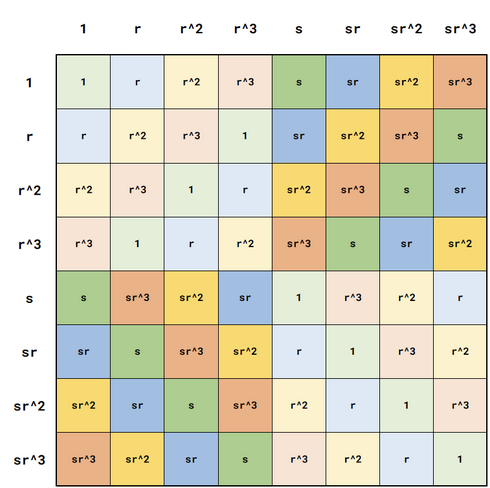
\includegraphics[scale=0.6]{cayleytable.png}
  \end{align*}
  \caption{The Cayley Table for the dihedral group $D_8$ is shown.}\label{fig:cayley}
\end{figure}

Computationally, we can select a unique element from the square's isometries consistently by
selecting the first element from the Cayley table of transformations. Alternatively, we can
generate the full set of the square's isometries. This table, shown in Fig.~\ref{fig:cayley},
represents the transformations of the dihedral group D generated by $<r,s\vert
  r^4=s^2={\left(sr\right)}^2=1>$. We treat the table like a set and filter another set containing
various arbitrary magic squares such that the resulting set only contains unique elements. This is
useful for brute-force algorithms where we may not have total control over element isometries in a
set. The same applies for certain constructive algorithms, but still, we ensure that we do not
duplicate magic squares in our sets, resulting in better analysis and more efficient runtimes.

\subsection{Factoring Magic Squares}

In the same manner that the dihedral group applied to the permutation of a square results in
the same square up to isometry, the dihedral group applied to a magic square always results in a
magic square. This property represents a symmetry of a magic square. Specifically, it represents
the rotational and reflective symmetry of an arbitrary magic square. Based on this, the application
of group actions on sets presents itself as a potential medium for representing group symmetry in
the magic square permutation group.

If we assume that the full set of magic squares is known, the group actions of the set would
be the full set of transformations between magic squares in the set. One thing we are interested in
is if these actions can tell us something new about the set that we didn't know before. Are there
additional magic-preserving sets of permutations, like those from the dihedral group? How many
symmetries exist for magic squares of a specific order? The answers to these questions may reveal
new patterns, lead to more efficient methods, or allow us to use smaller search-spaces for larger
orders.

Computationally, we can produce a transformation between two magic squares, $\pi$ and $\sigma$, by
factoring out the permutation $\alpha$ that acts on $\pi$ to produce $\sigma$. The factorization of
permutations is a well known problem and is computed by inverting part of the original composition.
The factorization method we use,~\boldmath{$\alpha=\pi^{-1}\sigma$}\unboldmath, stands as a
pivotal and indispensable step in laying the groundwork for the subsequent sections of this paper.
The full set of factors $\beta$ in a set of permutations can be computed by \boldmath{$\beta =
    \{\pi,\sigma\in S | \pi^{-1}\sigma\}$}\unboldmath.

Typically, when faced with actually computing magic squares, we only have access to subsets of
$M_n$. We denote an arbitrary subset of $M_n$ as $K_n$, more specifically, $K_n \subseteq M_n$.
Many methods for computing magic squares exist. As such, various distinct subsets are possible.
Regardless of the methods used, the group actions still may reveal information about $M_n$ despite
its incompleteness. We believe that additional magic squares can be extrapolated based on the
existing knowledge gained from analysis of its actions, products, and inverses.

\section{Solving Magic Squares}

\subsection{Introduction}

Ideally, we would like to have enough information about $M_n$ so that by computing one magic
square, we can generate $M_n$. This generally is the case for order three, considering there is
only one solution. However, this is not very interesting. For order four, there are 880 unique
solutions up to isometry, so we should expect to have to compute more than one magic square to
generate the full set of solutions in $M_4$. In practice this seems logical, considering there
isn't much that two arbitrary magic squares have in common besides their group properties. We will
have to dig deeper in order to find patterns amongst elements in $M_n$.

It should also be noted that the elements of $\beta$ are typically never magic. The idea is
that given an action $\alpha$ in $\beta$, and a magic square $\pi$ from $K_n$, then $\pi\alpha$ may
potentially be a new magic square, not already in $K_n$. Not all elements of $\beta$ produce magic
squares on elements of $K_n$. Discovering the space of solutions given an action is something we
wish to explore. One reason for this is that certain magic squares may exist in distinct cosets
that have a distinct permutation or permutations that act on it. These cosets may provide some
hints about the symmetries on $M_n$.

\subsection{Current Method}

Solving magic squares and producing the set $K_n$ is itself a different problem.
Programmatically, we use Rust in a multithreaded environment to squeeze out as much performance as
we can. We also utilize message passing on a single process, specifically, a Multiple Producer,
Single Consumer (MPSC) Queue to produce results on all threads available to the system. This method
is widely used in parallel systems that enable data communication primitives. In Rust, we are able
to do this very easily.

These results are then collected into a set-like data structure. We will use a
\texttt{BTreeSet} (Balanced Binary Search Tree) to store our magic squares for the fast lookup,
insertion, and concurrency potential. For our initial proof of concept, we first computed the first
440 magic squares of order four. This computation took about 40 minutes on 16 threads, each running
at 4.2 GHz. Of these 440 magic squares, 239 are unique. Notably, 239 is prime. Based on the time
taken to compute the initial set, we anticipate that a full brute-force computation of $M_n$ would
require about 10.67 hours.

\subsection{New Method}

We begin by reading the set of 440 cached magic squares as permutations, which we computed
previously. We then filter the set to reduce duplication, hence the resulting set only contains
unique squares up to isometry. The resulting unique set, in our case, contains 239 permutations,
and we will consider this set as $K_4$ where $K_4\subset M_4$. Up to this point, we have only
defined $K_4$ as a set containing 239 magic squares as permutations in relative order. It should be
noted that these are not necessarily the first 239 unique magic squares in lexicographical order
since our original $K_n$ was produced by multiple threads and at different rates, but we will
eventually explore this difference in our analysis.

Once $K_4$ is computed, we may then start producing the factors that act on $K_4$. We compute
the set of actions $\beta$ with $S = K_4$, so  $\beta = \{\pi,\sigma\in K_4| \pi^{-1}\sigma\ =
  \alpha\}$. The set $\beta$ contains the factors between all pairs of elements in $K_4$. Filtering
out isometries, this set contains 22,490 permutations.

Now, compute the full set of trivial isometries for all permutations in $K_n$ which we call
$Iso(K_4)$. Simply, this is the set of all rotations and reflections of the magic square
permutations in $K_4$ where $K_4\subsetneq Iso(K_4)$ and $|Iso(K_4)| = 8|K_4|$.

Then, we compute the product $Iso(K_4)\times\beta = \{\pi\in Iso(K_4),\alpha\in\beta |
  \pi\alpha \text{ is magic}\}$. For each permutation in $Iso(K_4)$ and for each $\alpha$ in
$\beta$,
if $\pi\alpha$ is magic, collect it into the set. If $\pi\alpha$ is not magic, do not collect it
and instead collect the action $\alpha$ into a set ${\beta}^\prime$.

Finally, we let ${K_4}^\prime = {K_4}^\prime \cup K_4$. What we have now is a set
${K_4}^\prime$ and ${\beta}^\prime$ where $K_4 \subseteq {K_4}^\prime \subseteq M_4$,
${\beta}^\prime \subseteq \beta$. For our specific set of permutations $K_4$, this algorithm yields
$|{K_4}^\prime| = |M_4| = 880 \Rightarrow K_4 \equiv M_4$ and $|\beta \setminus{\beta}^\prime| = 4$
after filtering out isometries.

\section{Analysis}

\subsection{Introduction}

The fact that $\left|K_4\right|< 880, \left|{K_4}^\prime\right|=880$ not only tells us that we've
found a great computational performance improvement, it also hints to us that there are possibly
more symmetries than just the 8 induced by the square isometries. These additional symmetries may
be key to producing more efficient algorithms as well as for making profound generalizations on
larger order magic square symmetry.

Overall, it will be very important for us to not only make statements based on experimental
data, but to back up our claims with logical reasoning. In any case, we will typically begin with
experimental data. The algorithm outlined in the previous section enables a greater range in
computational capability, however, it also opens a door to a whole new set of questioning regarding
the structure of the solution space for $M_4$. One of the things we would like to do with this
information is to understand why we are able to exploit magic square symmetry in this way so that
we may apply the same or similar methods for larger orders.

\subsection{Computational Analysis}

The result of ${K_4}^\prime$ with $\left|K_4\right|=239$ computes in 71 seconds. This is an
amazing computational performance improvement over the remaining 10 hours for brute-force
enumeration. The code is parallel across threads, thus we may conclude that the implementation
we've chosen is adequate. Of course, the sizes of the sets we work with are still rather large.
Only now, we may start to consider memory and storage as our most limiting factors. As
$\left|K_n\right|$ approaches $\left|M_n\right|$, the amount of memory required to continue working
with the sets grows extremely fast. In one case, we used $M_n$ as our $K_n$ and the program ran out
of memory. This is suboptimal, considering we would like to be able to use this algorithm to
compute large orders with minimal information.

The simplest solution to this is additional parallelization, although there also exists the
possibility for set partitioning. Additionally, we could revisit how the sets are represented
computationally to use more efficient implementations at this particular scale.
The combination of these solutions lands the problem in the realm
of High-Performance Computing (HPC) for proper multiprocess computation using extremely high CPU
counts, super-scale storage solutions, and vast quantities of working memory. Given our current
time and budget constraints, we see partitioning as the most viable solution to cutting down on the
memory/storage requirement at the cost of program runtime.

The amortized runtime analysis of the algorithm is difficult considering the amount of
abstraction used in the body of the code. Given that we compute (approximately) $\beta$ by $K_n
  \times K_n$ and $\beta \times K_n$, we may say the algorithm runs at approximately
$O\left(n^c\right)$ where $c$ is a constant. This beats the performance of iterative brute-force
which is
$O\left(n!\right)$. With this in mind, the set reduction incurred by looking at group actions in
this way is likely vast. The largest possible set with $n=239$ is $\approx 1.36519 \times 10^7$
whereas $16!\approx 2.09227 \times 10^{13}$.

\subsection{Generating Sets}

While the maximum set size difference is great for $n=239$, it is entirely dependent on our
choice of $K_n$. In a way, the choice of $K_n$ is completely arbitrary. We will choose a different
set now, also calling it $K_4$, however, we will select the first 440 magic squares from $M_4$ in
lexicographical order. This set contains 232 unique magic squares, produces a set of 20,210
actions, but only generates 871 unique magic squares from ${K_4}^\prime$. This is interesting since
it
is the first choice of $K_4$ that actually fails to compute $M_4$. What if we chose a different set
using a different sampling method?

One of our hypotheses was that certain types of magic squares have different kinds of
influence on the output of ${K_4}^\prime$, and we thought it could be related to the order of the
permutations in the set. Specifically, the order of a permutation is the \texttt{lcm} of all its
cycle lengths and represents the smallest integer $n \ni p^n = e$. Given our assumption, we
selected four elements from each conjugacy class and ran the resulting set through our algorithm,
producing ${K_4}^\prime$. The input set was small, only 104 elements, yet still produced $M_4$.
Following this, elements were iteratively removed from the set via backtracking if $M_4$ could
still be computed without them. The resulting set contained only 50 elements and ${K_4}^\prime$
still resulted in $M_4$. This discovery was extremely valuable since we could now compute $M_4$
from 50 magic squares alone with a total run time of about 1 second.

Initially, we were not entirely sure what the smallest set $K_n$ that produces $M_n$
represented. Our main theory was that the elements in the minimal set are
representatives of the cosets of $M_n$, where each element encodes with it some type of group
symmetry. If this is the case, then the minimal set possibly could contain fewer than 50 elements,
dividing the order of the group (due to Lagrange's theorem). Attempts at Monte Carlo simulation to
find smaller sets were not successful due to time constraints, but did suggest that the size of the
minimal set is very close to 50.

However, revisiting our definitions tells us that $K_n$ is a set of generators for a group
containing the elements of $M_n$. This implies that the smallest set $K_n$ that produces $M_n$ is
considered a ``minimal set $S$ that generates $G$'' which we  use interchangeably with ``generating
subset of minimal cardinality''. For finite, solvable groups, the cardinality $k$ of the minimally
generating subset is at least $\lceil\log_{p}{\left|G\right|}\rceil$ (where $p$ is the smallest
prime dividing $G$), which is a byproduct of Lagrange's Theorem\cite{Arvind}. Using the ``Groups,
Algorithms, and Programming'' system (GAP), an open-source programming model for computational
discrete algebra, we found that the group containing all magic squares of order four has an order
of 10,461,394,944,000 $\left(\frac{16!}{2}\right)$, which is equal to the order of the group
generated by our small $K_4$\cite{GAP4}. This may indicate that these groups are identical. With
$p=2$,
$\left|G\right|$=10,461,394,944,000, we found that the minimal cardinality of the subset that
generates $G$ is 44 (rounded up to the nearest integer).

In other words, the group containing all magic squares of order four requires that our initial
generating set contain at least 44 magic squares as generators, assuming our group is finite and
solvable. This is very close to the size of our small set ($\left|K_n\right|=50$). Finding a
group's minimally generating subset, whose length is the rank of the group, would allow us to more
accurately describe the group's structure, relationships, and dependencies amongst elements of the
group. The process for actually describing a generating set with minimal cardinality is still quite
difficult, even for computational approaches. In general, it's easiest to use methods that don't
require a total enumeration of the group. Also known as the Rank Problem, the concept of computing
a generating subset of a group with minimal cardinality is one of the most well known and
challenging problems in algorithmic group theory\cite{Baumslag}.

One other hypothesis we had is that different sampling methods or random distributions may
allow us to build more interesting sets to use as $K_n$. The relative distance between elements in
the set of 50 magic squares appears random \textemdash{} the set contains no discernible pattern.
Our
code implements some functionality that enables random sampling from $M_n$ using various
distributions. The main goal of testing different distributions is to explore the relative variety
generated by using different sampling methods. Of course, the next easiest method would be to build
$K_n$ from the various constructive algorithms that exist for magic squares. It would be
interesting to see what kind of variety and sampling distributions of $M_n$ we can achieve by using
certain algorithms to produce small sets of solutions as well as what effect this has on the output
of ${K_4}^\prime$.

\subsection{Magic-Preserving Group}

The action of the dihedral group on any magic square will always result in a magic square.
This is true for all magic squares, since the actions of rotating and reflecting a square are
magic-preserving. Similarly, other kinds of transformations exist that when applied to a magic
square, also produce a magic square. This group, in the context of group actions on sets and
element transformations, reveals a high degree of symmetry and can be used to further improve the
computational performance of enumerating magic squares.

Recall that we collect the actions
that fail at least once to produce a magic square when applied to $Iso(K_4)$. This set of actions,
${\beta}^\prime$, contains the set of counterexamples, assuming all actions $\alpha\in\beta$ result
in a magic square when we compute $\pi\alpha$ for $\pi\in Iso(K_4)$. Thus,
$MP=\beta\setminus{\beta}^\prime$ is the set of all actions, that when applied to $\pi\in
  Iso(K_4)$, are guaranteed to result in a magic square. To our surprise, $\left|MP\right|=4$
unique
up to isometry, implying three new magic-preserving symmetries in addition to the identity element.
These permutations as squares are:

\begin{figure}[ht!]
  \begin{align*}
    \begin{tabular}{|
      *{4}{>{\collectcell\fwcell}c<{\endcollectcell} |} }
      \hline 1  & 2  & 3  & 4  \\
      \hline 5  & 6  & 7  & 8  \\
      \hline 9  & 10 & 11 & 12 \\
      \hline 13 & 14 & 15 & 16 \\
      \hline
    \end{tabular}
    \quad
    \quad
    \quad
    \begin{tabular}{|
      *{4}{>{\collectcell\fwcell}c<{\endcollectcell} |} }
      \hline 1  & 3  & 2  & 4  \\
      \hline 9  & 11 & 10 & 12 \\
      \hline 5  & 7  & 6  & 8  \\
      \hline 13 & 15 & 14 & 16 \\
      \hline
    \end{tabular}
  \end{align*}
  \begin{align*}
    \begin{tabular}{|
      *{4}{>{\collectcell\fwcell}c<{\endcollectcell} |} }
      \hline 7  & 5  & 8  & 6  \\
      \hline 15 & 13 & 16 & 14 \\
      \hline 3  & 1  & 4  & 2  \\
      \hline 11 & 9  & 12 & 10 \\
      \hline
    \end{tabular}
    \quad
    \quad
    \quad
    \begin{tabular}{|
      *{4}{>{\collectcell\fwcell}c<{\endcollectcell} |} }
      \hline 7  & 8  & 5  & 6  \\
      \hline 3  & 4  & 1  & 2  \\
      \hline 15 & 16 & 13 & 14 \\
      \hline 11 & 12 & 9  & 10 \\
      \hline
    \end{tabular}
  \end{align*}
  \caption{The following squares are members of the magic-preserving group.}\label{fig:preserving}
\end{figure}

It is proven computationally that $\forall\pi\in\ M_4,\alpha\in MP, \pi\alpha \in M_4$. One
question that arises from the knowledge of this set is on whether $\pi\alpha$ should still be
considered uniquely as $\pi$, since this is how we treat the actions of the rotation and reflection
isometries on $\pi$.

\subsection{Additional Observations}

Our code also makes note of permutation parity as it relates to computations on permutations
of magic squares. The parity of a permutation $\pi$ is \texttt{even} if the sign function
$sgn\left(\pi\right)=1$. The sign function is defined as ${\left(-1 \right)}^k$ where $k$ is the
total number of disjoint transpositions of the permutation $\pi$. It is surprising to us that all
magic squares in $M_4$ map exclusively to even permutations in $S_n$. The set of all even
permutations in $S_n$ forms a subgroup of $S_n$ and is called the Alternating Group or
$A_n$. The order of $A_n$ is $\frac{n!}{2}$ which is the order of $\left\langle M_4 \right\rangle$.
Formally, we might be able to prove that $\left\langle M_4 \right\rangle \cong A_{16}$. Doing so
would allow us to better understand the subgroup structure of $\left\langle M_4 \right\rangle$, but
we leave this as an exercise for the reader.

\section{Conclusions}

\subsection{Introduction}

While confident in the performance of our new algorithm for solving magic squares, we have yet
to fully understand the implications of using magic squares in a group-theoretic context. The
application of a group structure to the set of magic squares of a specific order makes the
intuition for computations simpler. However, it also adds a significant amount of complexity and
increases the number of assumptions we use to compute them.

\subsection{Alternative Methods}

Compared to alternative methods for computing magic squares, we recognized very few approaches
that use a similar permutation group representation. Some of our initial assumptions and
applications of group theory almost transform the grid-square construction into a different kind of
problem, so we find it somewhat difficult to make direct comparisons to more standard models of the
magic square problem. In the few examples we found of solving magic squares using group theory, we
found that researchers tended to apply general linear group structures over permutation groups.
While this is a completely different approach, bringing with it other kinds of questions and
results, this is a perfectly valid way to go about solving magic squares as the information in
general linear groups is more geared towards grid/matrix problems, and thus contains a more
intuitive structure. Standard models, however, are typically very well-defined and date back to
some of the earliest research into the magic square puzzle. Oftentimes these standard models use
methods on magic squares that do not encapsulate the full solution set, rather, they typically aim
to produce magic squares in the most efficient/intuitive way regardless of the specific value of a
solution. This can be useful still, in cases where one only needs a solution, not necessarily
information about the space of all solutions.

\subsection{Generalizations}

For almost all of our examples, the algorithm we used to generate the complete set of magic
squares was implemented for order four. One generalization that we've considered and would like to
see, is if this algorithm can successfully be applied to magic squares with orders greater than
four. The code for this algorithm was designed to be order-agnostic meaning that, in theory, we
could very easily just use a different order of magic square and the same processes and
computations would still be applied to potentially generate the full set of solutions. Of course,
this assumes that solutions of magic squares of different orders can be computed using the same
transformations as order four.

We tested this on magic squares of order five but due to the sheer size of the solution space
for brute force calculations, we were unable to obtain a large enough initial generating set to
produce new terms. Our hypothesis is that with additional known magic squares of order five, we may
be able to generate additional solutions using our method. The same could potentially be said for
magic squares of order six and above, if proven to be true for smaller orders.

Additionally, we are curious if this algorithm still yields solutions for other kinds of magic
squares. For example, does removing the constraint on the diagonals affect the way permutations
interact with one another in a group structure? What about for pandiagonal magic squares?
Generalizing our algorithm for other kinds of magic squares could introduce more or less complexity
depending on the assumptions that other types of magic squares make. They could also yield wildly
different results based on their own group structure analysis.

\subsection{Open Questions}

Aside from the questions induced by thinking about potential generalizations of our
algorithm, there are still some things we don't know but would find useful in our discovery. Many
questions that we've had depended on the individual assumptions we've made up to that point.
Eliminating or potentially proving our assumptions will almost certainly improve our results.

\textbf{Does random sampling from a given distribution improve the relative variety of our
  generators over normal methods?} Given the difficulty of finding a minimally generating set, we
would like to know to what degree randomness could affect our ability to create smaller or
``stronger'' generating sets.

\textbf{To what degree might ``supercomputing'' improve our results?} This sort of problem could be
geared more for high-performance or massively distributed systems. Our code itself is actually
thread-agnostic in some cases which could enable increased performance and throughput of
computations.

\textbf{Are there better ways to represent magic squares as algebraic objects?} Our paper suffers
from formality. Since developing the algorithm in code was always a priority over formalization of
the underlying mathematics, our terminology and definitions might inadvertently be limiting our
ability to perform efficient analysis.

\textbf{How do the subgroup structures of $\left\langle M_4 \right\rangle$ generalize?} We noticed
a relationship between $\left\langle M_4 \right\rangle$ and $A_{16}$. Does this relationship
persist for all $n$ or is it only true for certain values? Specifically, is it true for all $n$
that $\left\langle M_n \right\rangle$ $\cong$ $A_{n^2}$?

\textbf{Are our results unique?} To our knowledge, our method introduces something new in the way
of solving magic squares, however we are not completely confident in its uniqueness according to
group theory. We believe with moderate confidence that our method uses results from theorems that
haven't necessarily been formalized in this paper.

% For an unnumbered remark, use the \texttt{xrem} environment.
% \begin{xrem} Note that \cref{low-bound} implies that there are infinitely many primes.
% \end{xrem}

\begin{thebibliography}{10}

  %items in the bibliography should be listed in alphabetical order
  %in order to ensure that your reference is formatted correctly, do the following:
  %   1) Visit mathscinet to find your citation; for example, search author=euclid, title=elements. Click on the citation
  %   2) Copy (ctrl-c) the reference from mathscinet; for example:
  %Euclid
  %Euclid's Elements.
  %All thirteen books complete in one volume. The Thomas L. Heath %translation. Edited by Dana Densmore. Green Lion Press, Santa Fe, %NM, 2002. xxx+499 pp. ISBN: 1-888009-18-7; 1-888009-19-5
  %01A75 (01A20 01A60 51-03)
  %   3) paste (ctrl-v) the reference into mref %https://mathscinet.ams.org/mref
  %   4) click search, then click TeX
  %   5) copy/paste the TeX code from mref as shown below:
  \bibitem{Andrews}
  Andrews, W.S. {\it Schrutka
      Literaturberichte: Magic squares and cubes}.
  Chicago, Court Publishing Co. 1908
  Monatsh. Math. Phys.20(1909), no.1, A57.
  MR1547984

  \bibitem{Arvind}
  Arvind V.
    {\it Some Algorithmic questions in Finite Group Theory}.
  \url{https://www.imsc.res.in/~knr/facets15/Slides/va.pdf}.
  Accessed: 2-17-2024

  \bibitem{Baumslag}
  Baumslag G;\@ Miller C. F.
    {\it Algorithms and classification in combinatorial group theory}.
  Papers from the Workshop on Algorithms, Word Problems and Classification in Combinatorial
  Group Theory held in Berkeley, California, January 1989.
  Math. Sci. Res. Inst. Publ., 23.
  Springer-Verlag, New York, 1992.\ viii+232 pp.
  MR1230626

  % \bibitem{Borowski}
  % Borowski, Ephraim J.; Borwein, Jonathan M.
  %   {\it Dictionary of Mathematics}.
  % University of California.
  % Collins (1989)

  \bibitem{Cammann}
  Cammann, Schuyler V. R.
    {\it The Evolution of Magic Squares in China}.
  Journal of the American Oriental Society, 80 (1960): 116.
  \url{https://www.jstor.org/stable/595587?origin=crossref}

  \bibitem{Cardelli}
  Cardelli, Luca; Wegner, Peter.
    {\it On understanding types, data abstraction, and polymorphism}.
  Computing Surveys, Vol 17 n. 4, pp 471-522, December 1985.
  \url{https://doi.org/10.1145/6041.6042}

  \bibitem{Deskins}
  Deskins, W.E.
    {\it Abstract Algebra}.
  {\it A series of advanced mathematics texts}.
  University of Michigan.
  Macmillan, 1964

  \bibitem{Fahimi}
  Fahimi, Peyman; Toussi, Cyrus Ahmadi; Trump, Walter; Haddadnia, Javad; Matta, Chérif F.
    {\it Striking patterns in natural magic squares' associated electrostatic potentials:
      matrices of the 4th and 5th order}.
  Discrete Math.344(2021), no.3, Paper No. 112229, 11 pp.
  MR4182931

  \bibitem{Fraser}
  Fraser, Craig G.
    {\it Chapter 19 - Joseph Louis Lagrange, Théorie des fonctions analytiques, first edition
      (1797)}.
  {\it Landmark Writings in Western Mathematics 1640-1940}.
  Edited by I. Grattan-Guinness Elsevier B. V., Amsterdam, 2005.\ xviii+1022 pp.
  MR2169816

  \bibitem{GAP4}
  {\it GAP - Groups, Algorithms, and Programming, Version 4.12.2}.
  The GAP~Group, 2022.
  \url{https://www.gap-system.org}

  \bibitem{Keough}
  Keough, Nathan.
    {\it Lo-Shu (crate)}.
  \url{https://github.com/natkeo559/lo-shu}

  \bibitem{Lehmer}
  Lehmer, D. H.
    {\it Teaching combinatorial tricks to a computer}.
  Proc. Sympos. Appl. Math., Vol. 10, pp. 179-193.
  American Mathematical Society, Providence, RI, 1960.
  MR0113289

  \bibitem{ONeill}
  O'Neill, Christopher.
    {\it The Weak Force Magic Square Order 6}.
  Cataphysics Group, 2021.
  DOI:10.13140/RG.2.2.26326.16965

  \bibitem{Wang}
  Wang J, Liu L.
    {\it A Novel Chaos-Based Image Encryption Using Magic Square Scrambling and Octree Diffusing}.
  Mathematics 2022, 10(3), 457.
  \url{https://doi.org/10.3390/math10030457}

  \bibitem{Weed}
  Weed Jared.
    {\it Applications of AI for Magic Squares}.
  eprint arXiv:1602.01401, 2016.
  \url{https://api.semanticscholar.org/CorpusID:119634667}

  \bibitem{Whitelaw}
  Whitelaw, Thomas A.
    {\it An introduction to abstract algebra}.
  Blackie, 1978.

\end{thebibliography}

\end{document}